%----------------------------------------------------------------------------
\chapter{Implementáció}
\label{chp:implementation}
%----------------------------------------------------------------------------
Ebben a fejezetben a fájlterítő alkalmazás implementációjának részeleteit mutatom be, mint annak követelményeit, konfigurálását, használatát, illetve felépítését.
Az alkalmazást Vmdistribution-nek neveztem el, forráskódja elérhető GitHub-on a cvswarrior/vmdistribution repository alatt\cite{vmdistribution}.

%----------------------------------------------------------------------------
\section{Követelmények és konfiguráció}
%----------------------------------------------------------------------------

A \textit{\textbf{Vmdistribution-t futtató}} gépen telepítve kell lennie a következőknek:
\begin{itemize}
  \item Egy JVM-nek\cite{stark2001java}, ami támogatja az 1.7-es verziójú Java-t(például az aktuális legfrissebb JRE az Oracle-től\cite{oraclejre}.).
  \item Vagrant 1.7.4, vagy frissebb
  \item Virtuális gépek kezelésére alkalmas szoftver - bármelyik Vagrant által támogatott\cite{vagrantproviders} (javasolt VirtualBox vagy VMWare Workstation használata)
\end{itemize}
Értelemszerűen azért van szükségünk JVM-re, hogy Java nyelven írodott alkalmazásokat tudjunk futtatni, Vagrantra és mondjuk VirtualBoxra pedig azért, hogy lehetőség legyen Vagrant által létrehozandó VM-ek terítésére.

A \textit{\textbf{labor}} gépeire vonatkozó követelmények:
\begin{itemize}
  \item Debian-alapú Linux disztribúció (természetesen a föggőségeket manuálisan fordítva tetszőleges disztribúció használható)
  \item SSH szerver engedélyezett jelszó alapú bejelentkezéssel
\end{itemize}
Az SSH szerverre azért van szükség, hogy tudjunk az összes laborgéppel kommunikálni, azokat távolról vezérelni, Debian-alapú disztibúcióra pedig, mert annak a csomagkezelezője segítségével van az alkalmazásunk függőségeinek nagy része telepítve.

A \textit{\textbf{labor}} gépeire a mellékelt telepítőszkriptek futtatásával, vagy manuálisan a következő alkalmazásokat kell telepíteni:
\begin{itemize}
  \item tmux
  \item rtorrent 0.9.6 vagy frissebb
  \item	sshpass\footnote{Csak azokon a gépeken szükséges, amiket terítéskor seed-nek akarunk használni}
  \item opentracker\footnotemark[1]
  \item apache (vagy egyéb XMLRPC protokollt kezelni tudó webszerver)
\end{itemize}
Az rtorrent tölti be a torrentkliens szerepét, az opentracker a tracker-ét, az apache segítségével tudja a gép a beérkező XMLRPC hívásokat fugadni és az rtorrent-nek továbbítani. Tmux segítségével tudunk távolról, szkriptből indított programot a ``háttérben'' futtatni, jelen esetben az rtorrent-et és az opentracker-t. Sshpass lehetőve teszi, hogy a seed gép jelszavas bejelentkezést használva automatizáltan tudjon SSH kapcsolatot létesíteni a többi laborgéppel.

%----------------------------------------------------------------------------
\section{Használat}
%----------------------------------------------------------------------------

Az alkalmazás használatához először is szükségünk van a labor modelljét leíró fájlra, ami tartalmazza annak felépítését és a lehetséges célállapotokat. Ezt legegyszerűbben az EMF által generált szerkesztővel lehet létrehozni. A program egy parancssori Java alkalmazás, ezért onnan a következőképpen indíthatjuk el:\\\\
\code{java -jar vmdistribution.jar modelfile goal\_lab logging\_level}\\\\
A 'modelfile' helyére értelemszerűen a modellt tartalmazó fájl elérési útvonala, a ``goal\_lab''-hoz a célállapotnak a neve, a ``logging\_level''-hez pedig a naplózási szint kerül. A naplózási szint alatt azt kell érteni, hogy mennyire részletes lesz a program futásának a kimenete, a lehetséges értékek részletesség szerinti növekvő sorrendben: WARNING, INFO, FINE, FINER.
A fájlterítés futását a STOP vagy S parancsokkal lehet megszakítani. Amennyiben véget ért a terítés a modellfájlban frissülni fognak a megfelelő Computer és VirtualMachine objektumok a terítés eredménye alapján.

%----------------------------------------------------------------------------
\section{Az alkalmazás felépítése}
%----------------------------------------------------------------------------

\begin{figure}[ht]
\centering
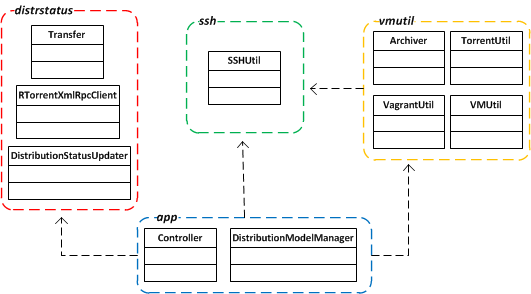
\includegraphics[width=150mm, keepaspectratio]{figures/packagediag.png}
\caption{}
\label{fig:packagediag}
\end{figure}

\begin{itemize}
  \item A funkcionalitás szempontjából jelentősebb osztályok bemutatása, komplexebb kódrészletek magyarázata
\end{itemize}

\definecolor{orange}{RGB}{255,127,0}
\definecolor{lightred}{RGB}{255,99,71}
\definecolor{seagreen}{RGB}{46,139,87}
\definecolor{skyblue}{RGB}{135,206,250}

\begin{center}
	\begin{tabular}{|>{\centering\arraybackslash}m{45mm}|>{\centering\arraybackslash}m{95mm}|}
		\hline
		\textbf{Osztály neve}&\textbf{Funkciójának rövid leírása}\\
		\hline
		\cellcolor{skyblue}UseModel & \cellcolor{skyblue}Az alkalmazás fő osztálya, ez tartalmazza main függvényt és vezérli a terítési folyamatot.\\ 
		\hline
		\cellcolor{skyblue}EMFModelUtil & \cellcolor{skyblue}A labor modelljét kezeli: betölti, futtatás után elmenti, illetve műveleteket tud végezni rajta (pl. kezdeti és végállapot közti különbség meghatározása\\
		\hline
		\cellcolor{seagreen}SSHUtil & \cellcolor{seagreen}SSH kapcsolatot tud létrehozni és azon keresztül távoli gépekre parancsokat küldeni és SCP protokollt használva fájlokat feltölteni.\\
		\hline
		\cellcolor{orange}VMUtil & \cellcolor{orange}Torrentfájlok létrehozására, seed-elés leech-elés indiítására.\\
		\hline
		\cellcolor{orange}TorrentUtil &\cellcolor{orange} \\
		\hline
		\cellcolor{orange}VagrantUtil &\cellcolor{orange} Vagrant alapú virtuális gépek inicializálására\\
		\hline
		\cellcolor{orange}Archiver &\cellcolor{orange} ZIP formátumú tömörített fájlok létrehozása\\
		\hline
		\cellcolor{lightred}RTorrentXmlRpcClient &\cellcolor{lightred} Kapcsolatot létesít XMLRPC protokollon keresztül a laborgépek torrentklienseivel\\
		\hline
		\cellcolor{lightred}DistributionStatusUpdater &\cellcolor{lightred} Torrentkliensektől kéri le való időben a terítés aktuális állapotát\\
		\hline
		\cellcolor{lightred}Transfer &\cellcolor{lightred} Egy VM->laborgép adatátvitelt reprezentál, tárolja a letöltés aktuális állapotát (mennyi van még hátra, sebesség stb.)\\
		\hline
	\end{tabular}
\end{center}

%----------------------------------------------------------------------------
\section{Egy konkrét terítés végigkövetése}
%----------------------------------------------------------------------------

A program 
+kis bevezető/apropó %TODO
A futatást a program fejlesztésére használt gépen végeztem el, a terítésben résztvevő gépek Vagrant-tal létrehozott, VirtualBox által futtatott virtuális gépek, amelyeken az operációs rendszer 32-bites 12.04 verziójú Ubuntu\cite{ubuntu}. A virtuális gépekre csak a legszükségesebb szoftverek lettek telepítve, egymással és a gazdagéppel egy közös privát hálózaton voltak. A program futtatásához megadott labormodell fontosabb paraméterei:

\begin{itemize}
  \item Két különböző virtuális gép van benne: egy mi általunk és egy Vagrant által készített
  \item 6 darab számítógép, amik közül az egyik dedikált seed (labpc101-105, seed nevűek)
  \item Olyan célállapot, amivel minden lehetséges hiba meg fog jelenni a futás során
\end{itemize}

Mielőtt végigkövetnénk a futtatást érdemes végiggondolni, hogy mi lenne az elvárt eredmény, milyen fontosabb lépéseket és milyen sorrendben fog a program végrehajtani:

\begin{enumerate}
  \item Figyelmeztetés, hogy 105 és 104-re semelyik, 103 és 102-re pedig egyik virtuális gép nem fog terülni bizonyos problémák miatt
  \item Vagrant-os VM inicializálása, majd becsomagolása egy .zip archívumba
  \item Mindkét VM felmásolása a seed gépre, mindkettőhöz torrent fájl létrehozása
  \item Torrentkliens futtatása a seed gépen
  \item Torrent fájlok átmásolása a labpc101-103 gépekre
  \item Torrentkliens futtatása a labpc101-103 gépeken
  \item A letöltések sikeres befejezése után a modell frissítése
\end{enumerate}

A program indítása után rögtön a várt figyelmeztetések jelennek meg a konzolablakban, például:\\\\
\code{2015-12-08 00:21:48 WARNING hu.bme.mit.vmdistribution.app.EMFModelUtil isCompatible WARNING:\_Computer:labpc104 is not compatible with Virtual Machine:vagrantvm\_test, Not enough RAM!}

Majd meghívódik a Vagrant és létrehozza, valamint beállítja a hozzá tartozó VM-et. \Aref{fig:vboxcap}-es~ábrán látható, hogy a VirtualBox VM-eket tartalmazó mappájába már bele is került az új virtuális gép és meg is jelenik annak a felületén.

\begin{figure}[ht]
\centering
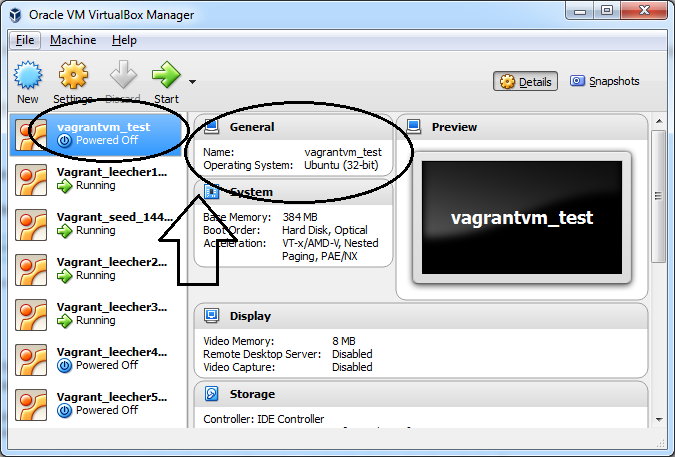
\includegraphics[width=140mm, keepaspectratio]{figures/test_vbox.png}
\caption{Vagrant által létrehozott virtuális gépek a VirtualBox-ban}
\label{fig:vboxcap}
\end{figure}
A kész virtuális gépből a program létrehoz egy tömörített .zip állományt\ldots\\\\
\code{2015-12-08 00:37:03 INFO hu.bme.mit.vmdistribution.app.vmutil.Archiver createZipArchive Creating Archive: E:\textbackslash{}vagrantvm\_test.zip}\\\\
\ldots majd a két VM felkerül a seed-re, ahogy \aref{fig:seed_files}-es~ábrán ez látszik is:  a seed-del SSH kapcsolat létesítése után kilistázzuk azoknak a mappáknak a tartalmát ahová a VM-eket tartalmazó zip fájlok, illetve az azok alapján készített torrent fájlok kerültek.

\begin{figure}[ht]
\centering
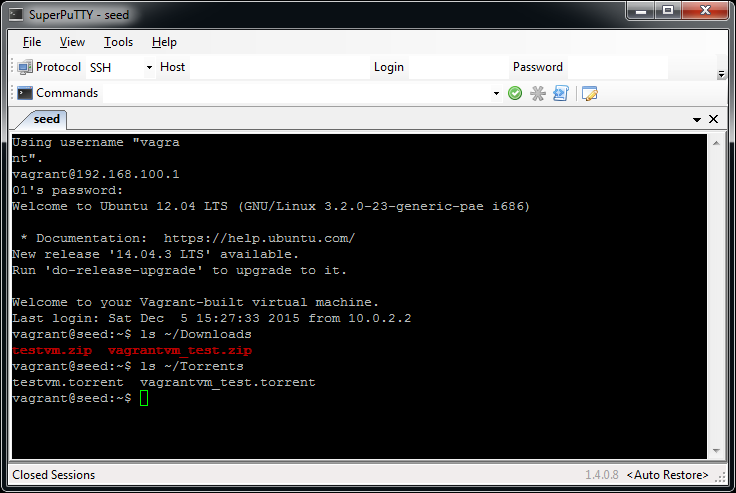
\includegraphics[width=140mm, keepaspectratio]{figures/test_seed_files.png}
\caption{Terítendő VM-ek és a torrent fájlok a seed-en}
\label{fig:seed_files}
\end{figure}

Ezután az alkalmazás a torrent fájlokat átmásolja a megfelelő célgépekre, és elindítja rajtuk a torrentklienst. A seed-en futó torrentklienst megnyitva ellenőrizhetjük, hogy elkezdődött-e az adatátvitel (\ref{fig:seed_torrent}. ábra). A feltöltési limit kézzel alacsonyra lett állítva, hogy a folyamatok megfigyelhetőek legyenek.

\begin{figure}[ht]
\centering
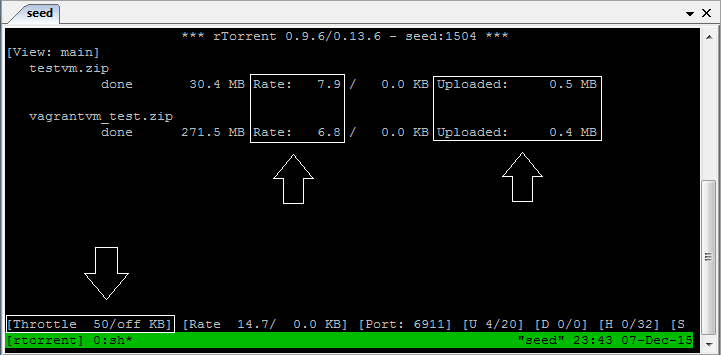
\includegraphics[width=140mm, keepaspectratio]{figures/test_seed_torrent.png}
\caption{Rtorrent: Futó feltöltések}
\label{fig:seed_torrent}
\end{figure}

A két futó fájlátvitel részleteit megnézve ellenőrizhetjük, hogy a megfelelő gépek töltenek-e le. Például a mi általunk készített VM-et tartalmazó testvm.zip-et a labpc101 és 103-nak kellene töltenie, lásd \ref{fig:seed_peers}-es~ábra (a két gép IP címe .111 ill. .113-ra végződik).

\begin{figure}[ht]
\centering
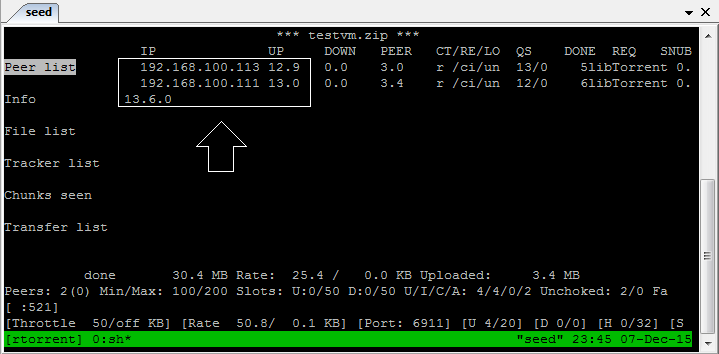
\includegraphics[width=140mm, keepaspectratio]{figures/test_seed_peers.png}
\caption{Rtorrent: Torrent részletei}
\label{fig:seed_peers}
\end{figure}

Egy pár percen belül véget is ér a terítés. A modellünket tartalmazó fájlt közelebbről megnézve ellenőrizhetjük, hogy az tényleg frissült-e, a labpc101-et reprezentáló Computer objektum például most már így néz ki:\\\\
\code{<computers virtualmachines="//@virtualmachines.1 //@virtualmachines.0" name="labpc101" maxSpaceForVMs="40000.0" installedRAM="8000.0" architecture="x64">}\\\\
A Computer-en levő virtuális gépeket a virtualmachines lista tárolja, aminek a két eleme a terített virtuális gépek objektumaira mutat.\\

+záró mondat %TODO
